%
% teil1.tex -- Beispiel-File für das Paper
%
% (c) 2020 Prof Dr Andreas Müller, Hochschule Rapperswil
%
% !TEX root = ../../buch.tex
% !TEX encoding = UTF-8
%
\section{Musterbildung in Reaktionsdiffusionssystemen
\label{reaktdiff:section:teil1}}

In diesem Abschnitt wird die Reaktionsdiffusionsgleichung mit zwei Komponenten untersucht.
Hierführ werden Turing-Muster betrachtet.
Turing-Muster findet man häufig in der Natur zum Beispiel als Fellmuster bei Tieren oder  das Muster unserer Fingerabdrücke.
Sie sind nach dem Mathematiker Alan Turing benannt, der sie 1952 in seinem Artikel \textit{The Chemical Basis of Morphogenesis} beschrieb.
Er untersuchte Systeme, die aus zwei Komponenten bestehen, einem Inhibitor und einem Aktivator.
Turing stellte für die entstehung der Turing-Muster eine Bedingung, die sogennante Turing Bedingung.
Sie besagt das ein System, in welchem Turing-Muster entstehen können, in abwesenheit von Diffusion stabil sein muss und mit Diffusion instabil wird.
Diese Kapitel basiert auf \cite{reaktdiff:turing_patterns_2019} \cite{reaktdiff:hoyle2006pattern}.

\subsection{Lineare Stabilitätsanalyse ohne Diffusion
\label{reaktdiff:subsection:mathe}}
Als Basis haben wir zwei Komponenten \(u\) und \(v\).
Die Reaktionsdiffusionsgleichungen für \(u\) und \(v\) lauten
\begin{align*}
    %\label{reaktdiff:equation:reaktdiff1}
    \frac{du}{dt} &= D_u \Delta u + f(u,v)\\
    \label{reaktdiff:equation:reaktdiff2}
    \frac{dv}{dt} &= D_v \Delta v + g(u,v)
\end{align*}
wobei \(D_u, D_v > 0\) die Diffusionskoeffizienten der Komponenten \(u\) und \(v\) sind.

Als erstes wird der erste Teil der Turing-Bedingung untersucht welche besagt das ein System ohne Diffusion Stabil sein muss.
Hierfür wird eine lineare Stabilitätsanalyse ohne Diffusion durchgeführt.
Man betrachte die Gleichungen
\begin{equation}
    \label{reaktdiff:equation:reaktdiff2ohneDiff}
    \frac{du}{dt} = f(u_0,v_0),\,
    \frac{dv}{dt} = g(u_0,v_0).
\end{equation}
Im fokus liegt die Stationärlösung \(u_0, v_0\) der Gleichungen \ref{reaktdiff:equation:reaktdiff2ohneDiff1},, das heisst das \(f(u_0,v_0) = g(u_0,v_0) = 0\).
Nun wird eine kleine Störung \(\epsilon\) zu \(u_0\) und \(v_0\) hinzugefügt.
\begin{align*}
    \delta u &= \epsilon u - u_0 \\
    \delta v &= \epsilon v - v_0.
\end{align*}
Die Störung \(\epsilon\) ist klein, das heisst \(\epsilon \ll 1\).
Jetzt kann man die Reaktionsterme linearisiern.
Hierfür nutzt man die Taylorentwicklung bis zum linearen Term.
Sie werden zu
\begin{align}
    f(u,v) &\approx f(u_0,v_0) + f_u \delta u + f_v\delta v\\
    g(u,v) &\approx g(u_0,v_0) + g_u \delta u + g_v\delta v.
\end{align}
Hierbei sind \(f_u, f_v, g_u, g_v\) die partiellen Ableitungen von \(f\) und \(g\) bezüglich \(u\) und \(v\).
Die Terme \(f(u_0,v_0)\) und \(g(u_0,v_0)\) sind Null, da \(u_0\) und \(v_0\) Stationärlösungen sind.
Nun können die Gleichungen \ref{reaktdiff:equation:reaktdiff2ohneDiff} umgeschrieben werden zu
\begin{align}
    \label{reaktdiff:equation:reaktdiff2ohneDifflinearisiert1}
    \frac{d \delta u}{dt} &= f_u \delta u + f_v \delta v\\
    \label{reaktdiff:equation:reaktdiff2ohneDifflinearisiert2}
    \frac{d \delta v}{dt} &= g_u \delta u + g_v \delta v.
\end{align}
Diese Gleichungen sind lineare partielle Differentialgleichungen.
Die Frage ist nun wie sich die Störungen \(\delta u\) und \(\delta v\) mit der Zeit entwickeln, werden sie grösser oder kleiner.
Wenn man sie als Matrixform screibt, erhält man
\begin{equation*}
    \label{reaktdiff:equation:reaktdiff2ohneDiffmatrix}
    \frac{d}{dt} \begin{pmatrix}
        \delta u\\
        \delta v
    \end{pmatrix} = 
    J 
    \begin{pmatrix}
        \delta u\\
        \delta v
    \end{pmatrix}
    , \quad
    J =
    \begin{pmatrix}
        f_u & f_v\\
        g_u & g_v
    \end{pmatrix}.
\end{equation*}

Die Matrix \(J\) ist die Jacobi-Matrix der Reaktionsgleichungen.
Damit die Gleichung stabil ist, müssen die Eigenwerte der Matrix \(J\) negative Realteile haben.
Hierbei ist es ausreichend dass die Spur \(\text{Tr}(J) < 0\) und die Determinante \(\det(J) > 0\) sind.
Das kann man zeigen, indem
\begin{equation*}
    \det(A - \lambda I) = 0
\end{equation*}
gelöst wird, wobei \(I\) die Einheitsmatrix ist.
Die Eigenwerte der Matrix \(J\) sind die Lösungen der Gleichung
\begin{equation*}
    \lambda^2 - \text{Tr}(J) \lambda + \det(J) = 0.
\label{reaktdiff:equation:reaktdiff2ohneDifflinearisiert3}
\end{equation*}
Die Eigenwerte der Matrix \(J\) sind die Lösungen der Gleichung
\begin{equation*}
    \lambda_{1,2} = \frac{1}{2} \left( \text{Tr}(J) \pm 
    \sqrt{\text{Tr}(J)^2 - 4 \det(J)} \right).
\label{reaktdiff:equation:reaktdiff2ohneDifflinearisiert4}
\end{equation*}
Hier sieht man das der Wert unter der Wurzel immmer kleiner ist als die Spur der Matrix \(J\) wenn die Determinante positiv ist.
Somit muss die Spur der Matrix \(J\) negativ sein, damit die Eigenwerte negative Realteile haben.

\subsection{Lineare Stabilitätsanalyse mit Diffusion
\label{reaktdiff:section:matheDiff}}
Nun wird die Diffusion in die Gleichungen \ref{reaktdiff:equation:reaktdiff2ohneDifflinearisiert2} und \ref{reaktdiff:equation:reaktdiff2ohneDifflinearisiert1} eingeführt.
Die Gleichungen werden zu
\begin{align}
    \label{reaktdiff:equation:reaktdiff2mitDiff1}
    \frac{d \delta u}{dt} &= D_u \Delta \delta u + 
    f_u \delta u + f_v \delta v\\
    \label{reaktdiff:equation:reaktdiff2mitDiff2}
    \frac{d \delta v}{dt} &= D_v \Delta \delta v + 
    g_u \delta u + g_v \delta v.
\end{align}
Damit die Turing-Bedingung für die Musterbildung erfüllt ist muss dieses System instabil sein.
Mit Diffusion wollen wir die Störungsentwicklung mit hilfe von Fourier untersuchen.
Dazu setzen wir \(\delta u(x,t) = c_k(t) e^{ikx} e^{\lambda t}\) und \(\delta v(x,t) = d_k(t) e^{ikx} e^{\lambda t}\) ein.
Die Ableitungen werden zu
\begin{align*}
    \frac{\partial\,\delta u}{\partial t} &= \sum_k \lambda\, c_k e^{i k x} e^{\lambda t}, &
    \Delta \delta u &= \sum_k -k^2 c_k e^{i k x} e^{\lambda t} \\
    \frac{\partial\,\delta v}{\partial t} &= \sum_k \lambda\, d_k e^{i k x} e^{\lambda t}, &
    \Delta \delta v &= \sum_k -k^2 d_k e^{i k x} e^{\lambda t}
\end{align*}
Setzen wir diese Ableitungen in die Gleichungen \ref{reaktdiff:equation:reaktdiff2mitDiff} ein, erhalten wir
    \begin{align*}
        \lambda c_k &= -D_u k^2 c_k + f_u c_k + f_v d_k \\
        \lambda d_k &= -D_v k^2 d_k + g_u c_k + g_v d_k
    \end{align*}
Die Gleichungen kann man wieder in Matrixform schreiben.
Somit erhält man
\begin{equation*}
    \lambda
    \begin{pmatrix}
    c_k \\
    d_k
    \end{pmatrix}
    =
    \begin{pmatrix}
        f_u - D_u k^2 & f_v \\
        g_u & g_v - D_v k^2
    \end{pmatrix}
    \begin{pmatrix}
    c_k \\
    d_k
    \end{pmatrix}
\end{equation*}
Kürzen wir die Gleichung durch \(c_k(t)\) und \(d_k(t)\) erhalten wir die Gleichungen
\begin{align}
    \label{reaktdiff:equation:reaktdiff2mitDiffFourierk}
    \lambda = J - k^2 D, \quad 
    J =
    \begin{pmatrix}
        f_u & f_v\\
        g_u & g_v
    \end{pmatrix}, \quad
    D =
    \begin{pmatrix}
        D_u & 0\\
        0 & D_v
    \end{pmatrix}.
\end{align}
Um die Gleichungen übersichtlicher zu schreiben, wird die Jacobi-Matrix \(J\) und die Diffusionsmatrix \(D\) in eine Matrix
\begin{equation}
    \label{reaktdiff:equation:reaktdiff2mitDiffFourierkA}
    A(k) =
    \begin{pmatrix}
        f_u - D_u k^2 & f_v\\
        g_u & g_v - D_v k^2
    \end{pmatrix}
\end{equation}
zusammengefasst.
Damit dieses System nun instabil ist muss der Realanteil der Eigenwerte der Matrix \(A\) positiv sein.
Das Ziel ist es nun die Eigenwerte der Matrix \(A\) zu bestimmen.
Um die Eigenwerte zu bestimmen muss man die Gleichung
\begin{equation}
    \det(A - \lambda I) = 0
\label{reaktdiff:equation:reaktdiff2mitDiffFourierkAeig}
\end{equation}
lösen, wobei \(I\) die Einheitsmatrix ist.
Das ergibt eine quadratische Gleichung in \(\lambda\):
\begin{equation}
    \lambda^2 - \text{Tr}(A) \lambda + \det(A) = 0.
\label{reaktdiff:equation:reaktdiff2mitDiffFourierkAeig2}
\end{equation}
Die Eigenwerte der Matrix \(A\) sind die Lösungen der Gleichung
\begin{equation}
    \lambda = \frac{1}{2} \left( \text{Tr}(A) \pm 
    \sqrt{\text{Tr}(A)^2 - 4 \det(A)} \right).
\label{reaktdiff:equation:reaktdiff2mitDiffFourierkAeig3}
\end{equation}
Somit hat man eine Formel mit der man für eine bestimmte Wellenzahl \(k\) die Eigenwerte \(\lambda\) bestimmen kann.
Aus der Gleichung \ref{reaktdiff:equation:reaktdiff2mitDiffFourierkAeig3} erhält man zwei Eigenwerte \(\lambda_1\) und \(\lambda_2\).
Wenn nun einer dieser Eigenwerte einen positiven Realteil hat, wird die Stationärlösung instabil.
Diese Instabilität ist verantworlich für die Musterbildung


\section{Bedingung für die Musterbildung
\label{reaktdiff:section:diffusioninduzierteInstabilitaet}}
Was in den vorhergehenden Abschnitten gezweigt wurde, ist das ein System ohne Diffusion stabil sein kann, aber mit Diffusion instabil wird.
Nun kann man aus den gemachten berechungen Bedingungen für die Musterbildung ableiten.
Einerseits muss die Stationärlösung stabil sein, das heisst die Spur der Jacobi-Matrix \(J\) muss negativ sein und die Determinante der Jacobi-Matrix \(J\) muss positiv sein.
Somit gilt
\begin{align*}
    \text{Tr}(J) &= f_u + g_v < 0, \\
    \det(J) &= f_u g_v - f_v g_u > 0.
\end{align*}
Andererseits muss die Diffusion so gewählt sein, dass die Eigenwerte der Matrix \(A\) mit der Wellenzahl \(k\) einen positiven Realteil haben.
Das geht wenn die Determinante der Matrix \(A\) negativ ist oder wenn die Spur negativ ist.
Somit gilt
\begin{align}
    \text{Tr}(A) &= f_u  + g_v - k^2(D_v + D_u)  < 0, \\
    \det(A) &= D_uD_vk^4 - (D_vf_u + D_ug_v)k^2 + f_u g_v - f_v g_u < 0.
    \label{reaktdiff:equation:reaktdiffbedingunen}
\end{align}
Da \(D_v,D_u > 0\) und der letzte Teil der Determinante positiv ist, muss der Ausdruck \(D_vf_u + D_ug_v\) positiv sein, damit die Determinante der Matrix \(A\) negativ ist.
Da \(f_u > 0\) und \(g_v < 0\) ist, muss auch
\begin{equation}
    \frac{D_v}{D_u}f_u > g_v
\end{equation}
damit die Determinante der Matrix \(A\) negativ ist.

Man sieht das die Deteminante von \(A\) ein Polynom 2. Grades in \(k^2\) ist.
Ausserdem representiert sie eine Parabel, die nach oben geöffnet ist, da der Koeffizient \(D_uD_v > 0\) ist.
Somit können wir die mininmale Wellenzahl \(k\) bestimmen, bei der die Determinante negativ ist.
Dafür leiten wir die Determinante nach \(k^2\) ab und setzen sie gleich Null.
Somit erhalten wir
\begin{equation*}
    \frac{d}{dk^2} \det(A) = 2D_uD_vk^2 - D_v f_u - D_u g_v = 0.
\end{equation*}
Die minimale Wellenzahl \(k\) ist also
\begin{equation*}
    k^2_{\text{min}} = \frac{D_vf_u + D_ug_v}{D_uD_v}.
\end{equation*}
Die minimale Wellenzahl \(k_{\text{min}}\) wird nun in die Gleichung für die Determinante der Matrix \(A\) \ref{reaktdiff:equation:reaktdiffbedingunen} eingesetzt.
Somit erhält man einen Ausdruck für den minimalwert Determinante welcher lautet
\begin{equation*}
    \det(A) = \frac{(D_v f_u + D_u g_v)^2}{D_u D_v} - f_u g_v - f_v g_u.
\end{equation*}
Die Determinante der Matrix \(A\) ist also positiv, wenn
\begin{equation*}
    \frac{(D_v f_u + D_u g_v)^2}{D_u D_v} - f_u g_v - f_v g_u > 0.
\end{equation*}
oder umgestellt
\begin{equation*}
    D_ug_v+D_vf_u < 2\sqrt{D_u D_v(f_u g_v - f_v g_u)}.
\end{equation*}
Das ist ein weiterer Bedingung für die Musterbildung in Reaktionsdiffusionssystemen.
Aus den Bedingungen kann man ein generelles System erkennen welches man Aktivator-Inhibitor System.
Hierführ ist die Vorzeichenstruktur der Jakobimatrix relevant.
Im klassischen Fall sieht sie so aus:
\begin{equation*}
        J =
    \begin{pmatrix}
        f_u & f_v\\
        g_u & g_v
    \end{pmatrix} 
    \rightarrow
    \begin{pmatrix}
        + & -\\
        + & -
    \end{pmatrix}
\end{equation*}
Die vorzeichen erfüllen folgende Eigenschaften:
\begin{itemize}
    \item \(f_u > 0\): Aktivator aktiviert sich selbst
    \item \(f_v < 0\): Inhibitor hemmt den Aktivator
    \item \(g_u > 0\): Aktivator aktiviert den Inhibitor
    \item \(g_v < 0\): Inhibitor hemmt sich selbst
\end{itemize}
Beispiele eines Aktivator-Inhibitor kann man in der Natur finden.
Ein Raubtier(Inhibitor) braucht Nahrung in form von Beutetiere(Aktivator) um zu überleben.
Jagen die Raubtiere zu viel haben sie zu wenig Nahrung.
Gibt es zu wenig Raubtiere vermehren sich die Beutetiere.
Die folge davon ist dass die Raubtiere sich ebenfalls vermehren bis wiederrum zu wenig Beutetiere vorhanden sind.
Dieses System reguliert sich selbst und hat eine stationäre Lösung.

Somit erhalten wir folgende Bedingungen für die Musterbildung:
        \begin{itemize}
            \item \(f_u > 0\): Aktivator aktiviert sich selbst
            \item \(g_v < 0\): Inhibitor hemmt sich selbst
            \item \(f_v < 0\): Inhibitor hemmt den Aktivator
            \item \(g_u > 0\): Aktivator aktiviert den Inhibitor
            \item \(\text{tr}(J) = f_u + g_v < 0\): Stabil ohne Diffusion
            \item \(\det(J) = f_u g_v - f_v g_u > 0\): Keine Eigenwertinstabilität ohne Diffusion
            \item \(D_u g_v + D_v f_u < 2\sqrt{D_u D_v (f_u g_v - f_v g_u)}\)
            \item \(D_v \gg D_u\): Inhibitor diffundiert deutlich schneller
        \end{itemize}


\subsection{Einfaches Beispiel}
Um das ganze an einem einfachen Beispiel zu zeigen werden
\begin{equation}
f(u, v) = a u + b v + k_1, \,
g(u, v) = c u + d v + k_2
\label{reaktdiff:equ:ownreakterm}
\end{equation}
als Reaktionsterme eingesetzt.
Als Parameter werden \( a = 1.0,\; b = -1.4,\; c = 1.0,\; d = -1.1,\; k_1 = 0.4,\text{und }k_2 = 0.1 \) eingesetzt.
Durch die Wahl von \(k_1\) und \(k_2\) befindet sich das Gleichgewicht bei \(u_0 = v_0 = 1\).
Nun werden die Bedingungen für die Musterbildung überprüft.
Hier führ berechen wir die Jakobimatrix
\begin{equation*}
        J =
        \begin{pmatrix}
        \frac{\partial f}{\partial u} & \frac{\partial f}{\partial v} \\
        \frac{\partial g}{\partial u} & \frac{\partial g}{\partial v}
        \end{pmatrix}
        =
        \begin{pmatrix}
        a & b \\
        c & d
        \end{pmatrix}
        =
        \begin{pmatrix}
        1.0 & -1.4 \\
        1.0 & -1.1
        \end{pmatrix}
\end{equation*}
Man sieht direkt das die Vorzeichenstruktur die eines Aktivator-Inhibitor Systems entspricht.
Nun benötigt man die Deteminante und die Spur.
Diese entprechen \(\det(J) = 0.3\) und \(\text{Tr}(J) = -0.1\).
Somit sind die Bedingungen \(\det(J) > 0\) und \(\text{Tr}(J) <0\) erfüllt.

Weiter geht es mit der Jakobimatrix mit Diffusion.
Die Determinante wird mit
\begin{equation*}
    \det(A(k^2)) = D_u D_v k^4 - (D_v a + D_u d) k^2 + \det(J)
\end{equation*}
berechnet.
Eine der Bedingungen ist das \(\det(A(k_{\min}^2))\) kleiner 0 ist.
Das minimum ist bei
\begin{equation*}
    k^2_{\text{min}} = \frac{D_v a + D_u d}{2 D_u D_v}
\end{equation*}
Da eine der Bedingungen \(D_v \ll D_u\) ist werden \(D_u = 1\) und \(D_v = 20\) gewählt.
Somit erhalten wir als minimum
\begin{equation*}
    k^2_{\text{min}} = \frac{D_v a + D_u d}{2 D_u D_v} = \frac{18.9}{40} = 0.4725
\end{equation*}
Setzen wir nun \(k^2_{\text{min}}\) in der Determinante ein erhält man
\begin{equation}
    \det(A) = 20k^4 - (20 \cdot 1.0 + 1 \cdot (-1.1))k^2 + 0.3 = 20k^4 - 18.9k^2 + 0.3
     = -4.165125.1
\end{equation}
Somit ist die Bedingung das die Deteminante mit Diffusion kleiner 0 wird erfüllt.
Ein System mit diesen Reaktionsterme wird Muster bilden.
Ein Beispiel ist in Abbildung \ref{reaktdiff:fig:ownreakterm} zu sehen.
In Abbildung \ref{reaktdiff:fig:easyfft} ist die Räumliche FFT zu sehen.

\begin{figure}
    \centering
    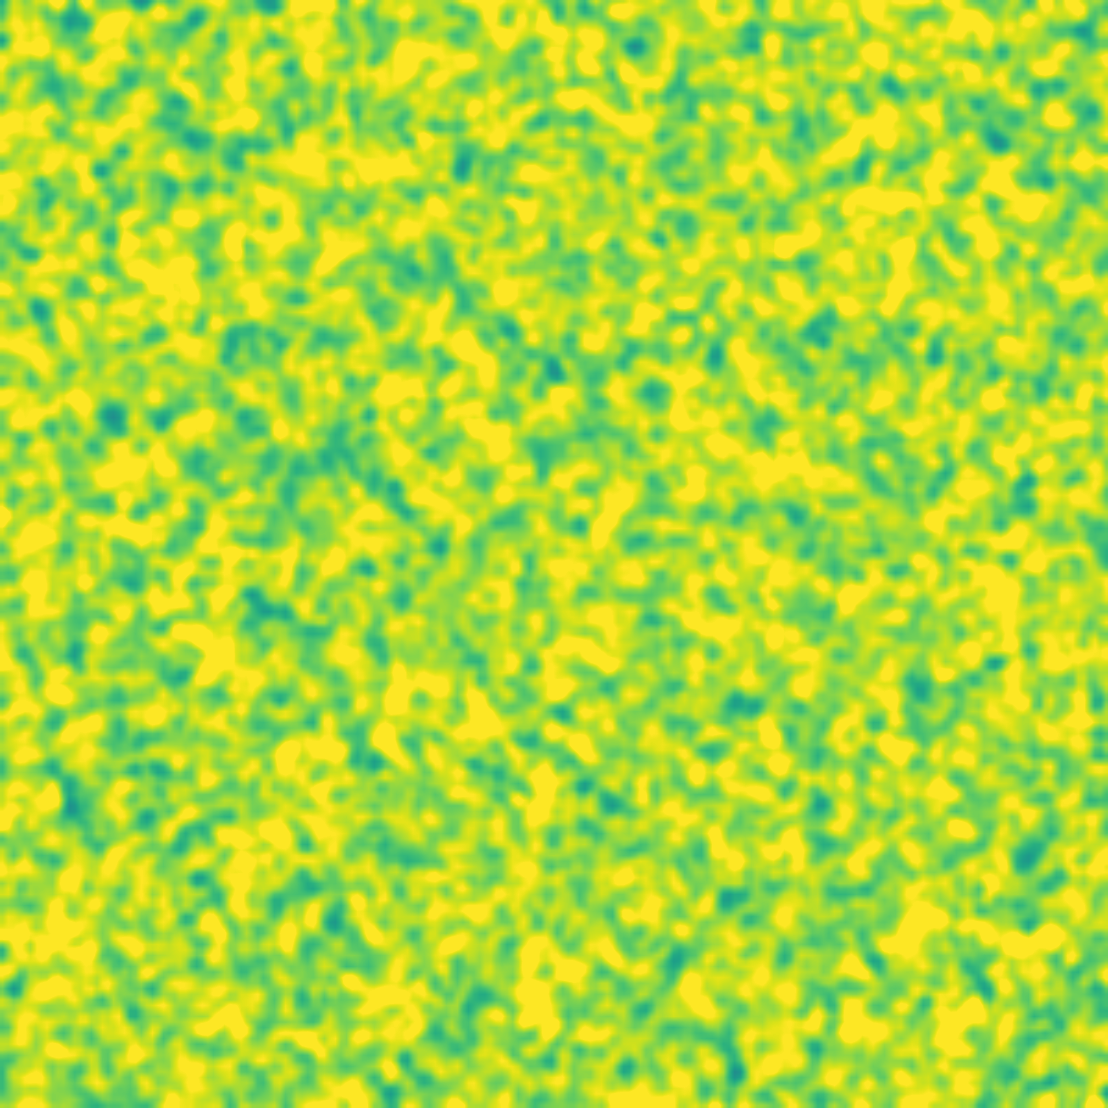
\includegraphics[width=0.32\linewidth]{papers/reaktdiff/images/simpleExample/easy_n1.png}
    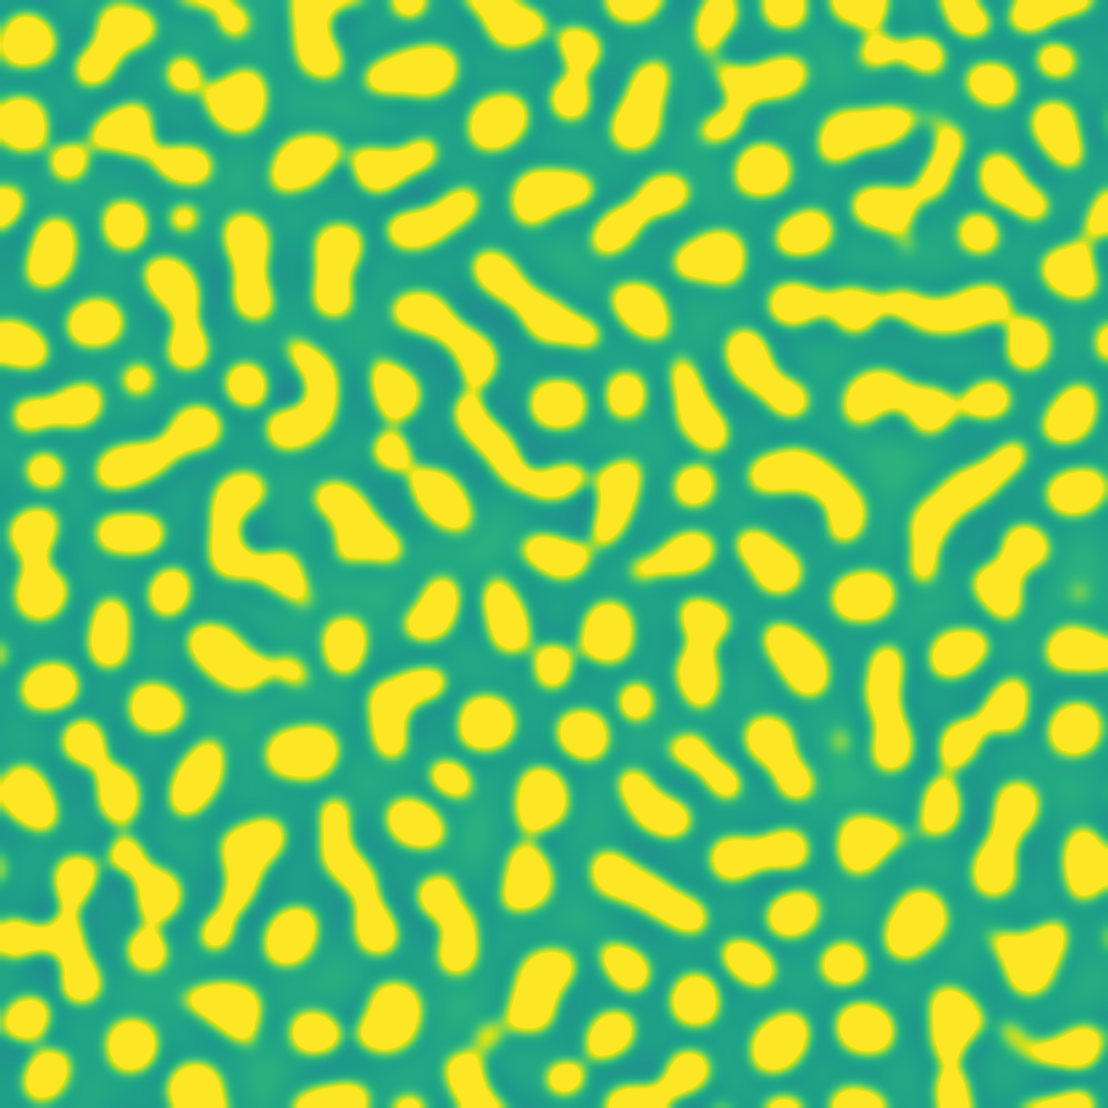
\includegraphics[width=0.32\linewidth]{papers/reaktdiff/images/simpleExample/easy_n300.png}
    
\includegraphics[width=0.32\linewidth]{papers/reaktdiff/images/simpleExample/easy_n999.png}
    \caption{Verlauf der Simulation (Links nach Rechts) der Reaktions-Diffusiongleichung mit \ref{reaktdiff:equ:ownreakterm} als Reaktionsterm}
    \label{reaktdiff:fig:ownreakterm}
\end{figure}

\begin{figure}
    \centering
    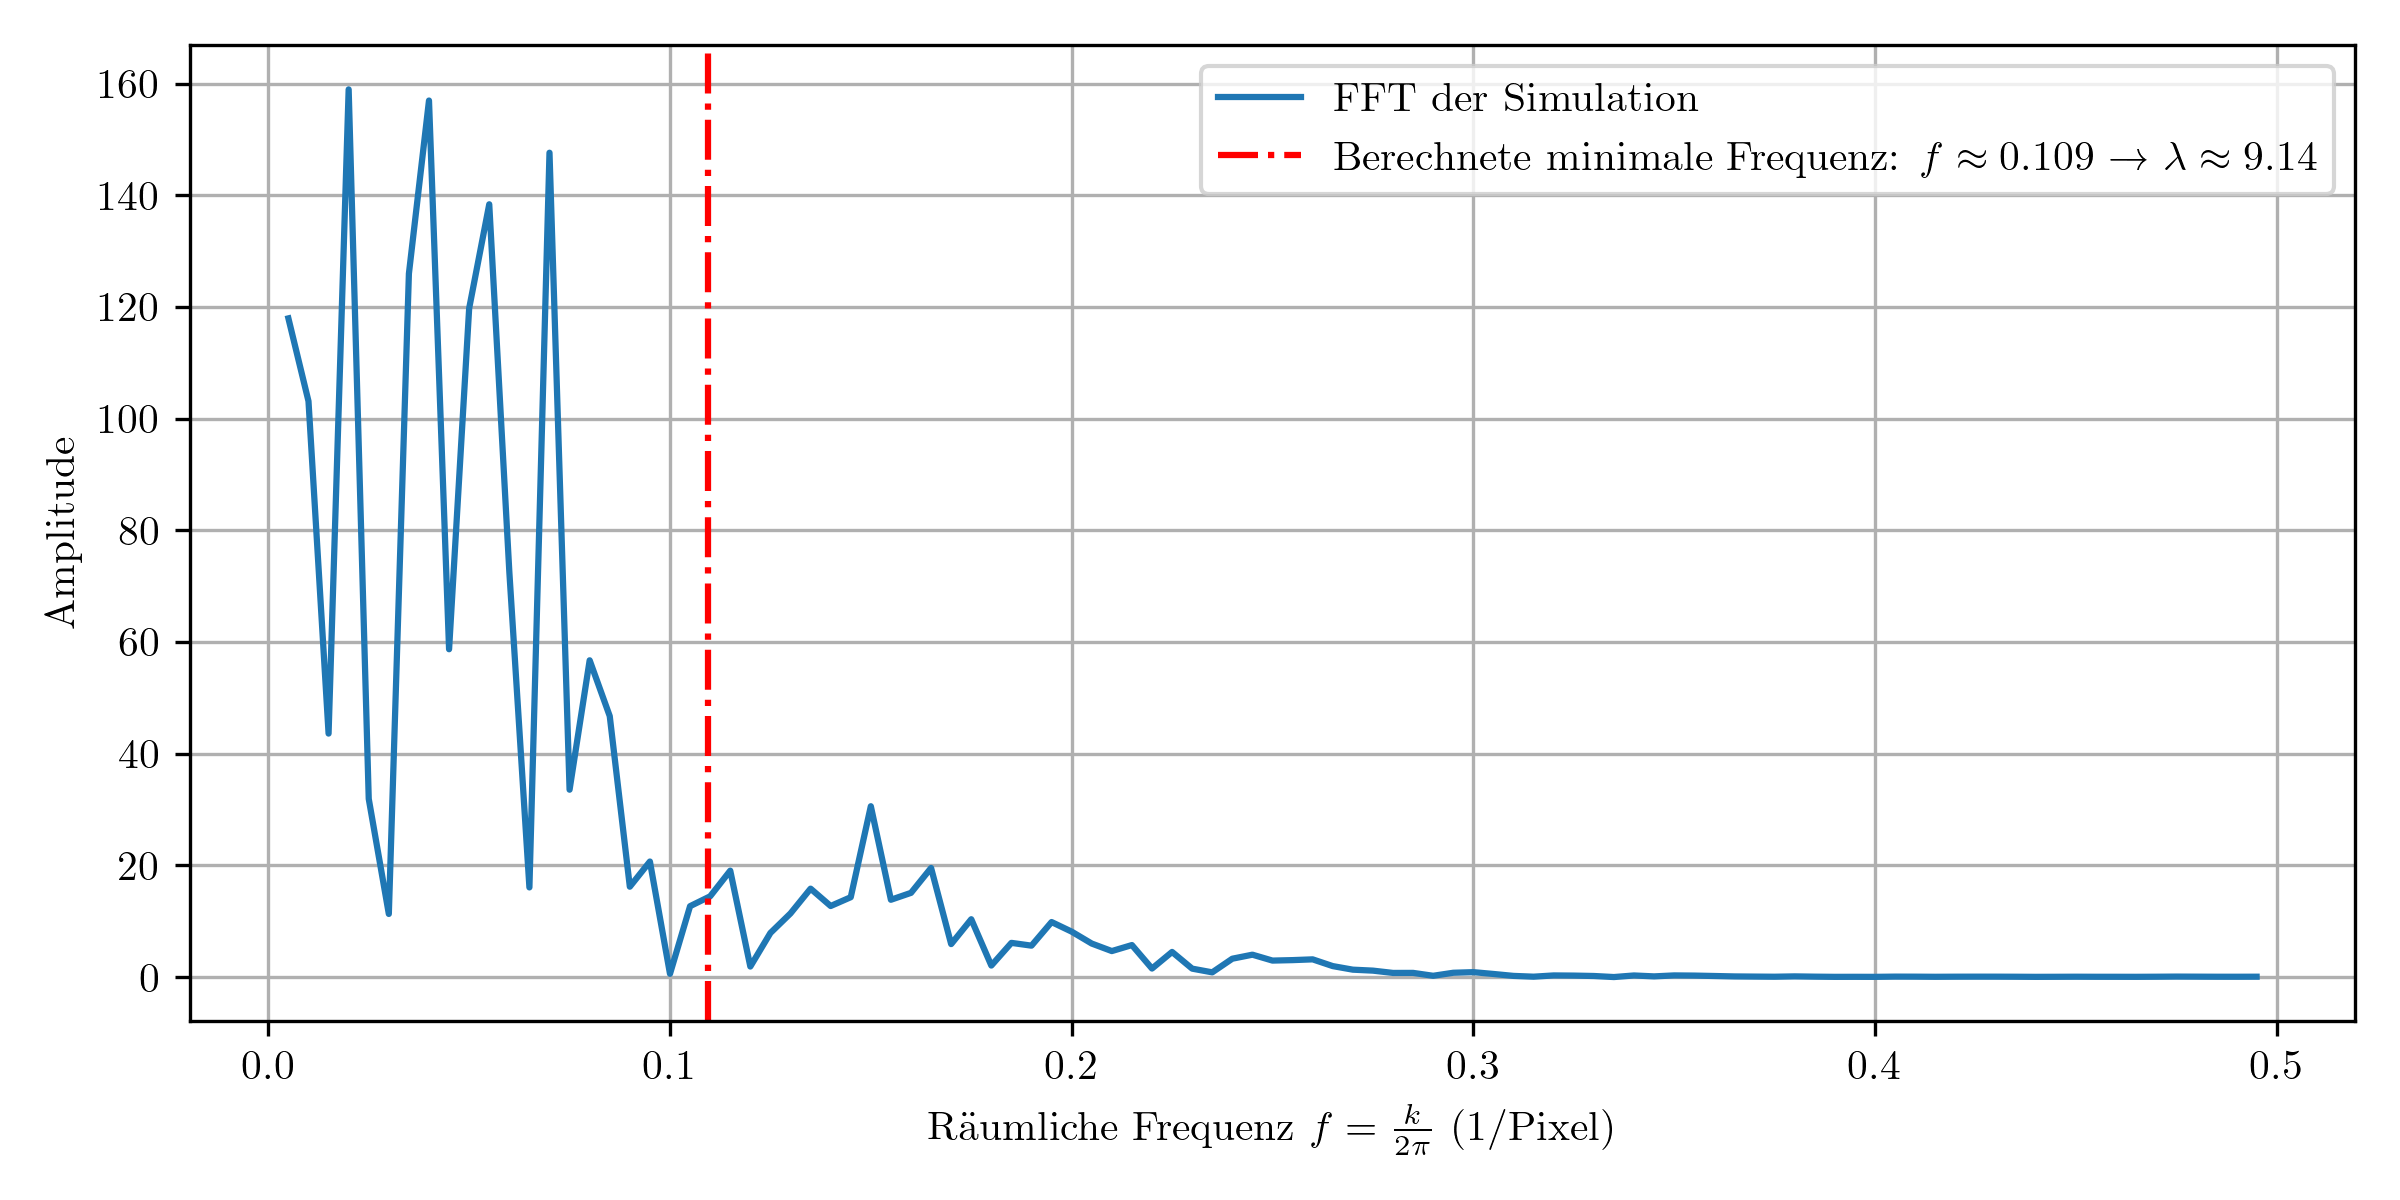
\includegraphics[width=\linewidth]{papers/reaktdiff/images/simpleExample/fft_turing_1d.png}
    \caption{FFT der Animation. Die rote Linie zeigt die theortische minimale Frequnez von \(f = k_{\min} / 2 \pi \approx 0.109\). Man sieht das die dominanten Frequnzen links des berechneten minimums ist.}
    \label{reaktdiff:fig:easyfft}
\end{figure}

%\begin{table}[h!]
%    \centering
%    \begin{tabular}{lcc}
%    \textbf{Größe} & \textbf{Theorie} & \textbf{Simulation (FFT)} \\
%    Dominante Frequenz $f$ (1/Pixel) & $\approx 0{,}075$ & $\approx 0{,060$ \\
%    Wellenlänge $\lambda = 1/f$ (Pixel) & $\approx 13{,}33$ & $\approx 16{,}67$ \\
%    Wellenzahl $k = 2\pi / \lambda$ & $\approx 0{,}472$ & $\approx 0{,}377$ \\
%    \end{tabular}
%    \caption{Vergleich zwischen theoretischer und numerisch bestimmter dominanter Wellenlänge. Die leichte Abweichung ist auf numerische Effekte der Simulation zurückzuführen.}
%    \label{tab:turing-vergleich}
%\end{table}



\subsection{Klasssische Reaktionsterme}
In der Literatur werden viele weitere Reaktionsterme erwähnt.
Eignige wenig werden hier im anschluss beleuchtet.
Die folgenden Bilder zu den Modellen sind mit finiten Differenzen erstellt worden.

Als ester wird das Gray-Scott Model berachtet.
Die Reaktionsterme
\begin{equation}
     f(u,v) = -uv^2 + F(1 - u), \quad g(u,v) = uv^2 - (F + k)v
     \label{reaktdiff:equ:fhn}
\end{equation}
fördern Wurmartigemuster.
Ein Beispiel kann in Abbildung \ref{reaktdiff:fig:fhn} gsehen werden
\begin{figure}
    \centering
    
\includegraphics[width=0.32\linewidth]{papers/reaktdiff/images/FitzHughNagumo/fhn_n1.png}
    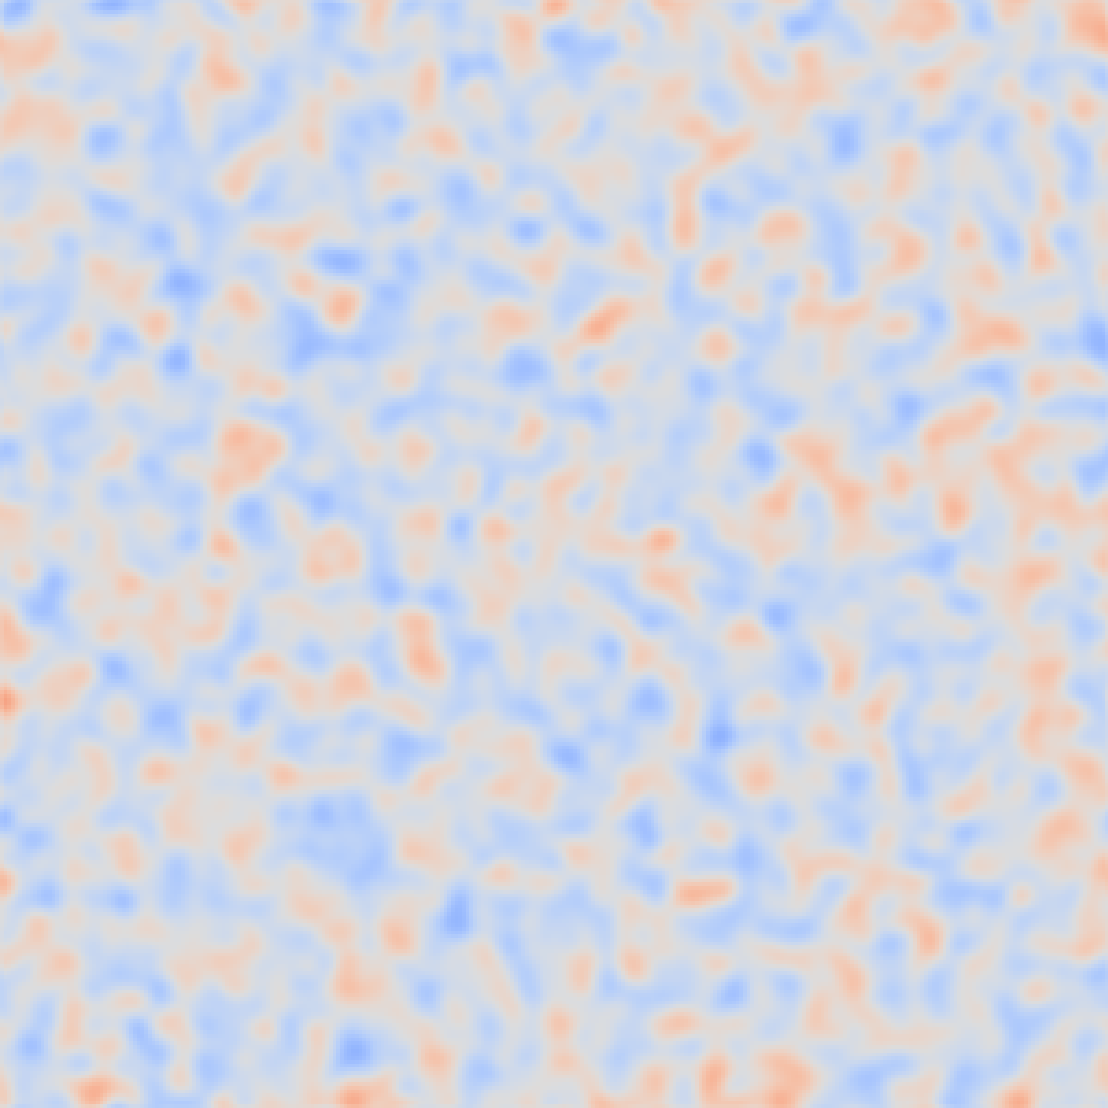
\includegraphics[width=0.32\linewidth]{papers/reaktdiff/images/FitzHughNagumo/fhn_n300.png}
    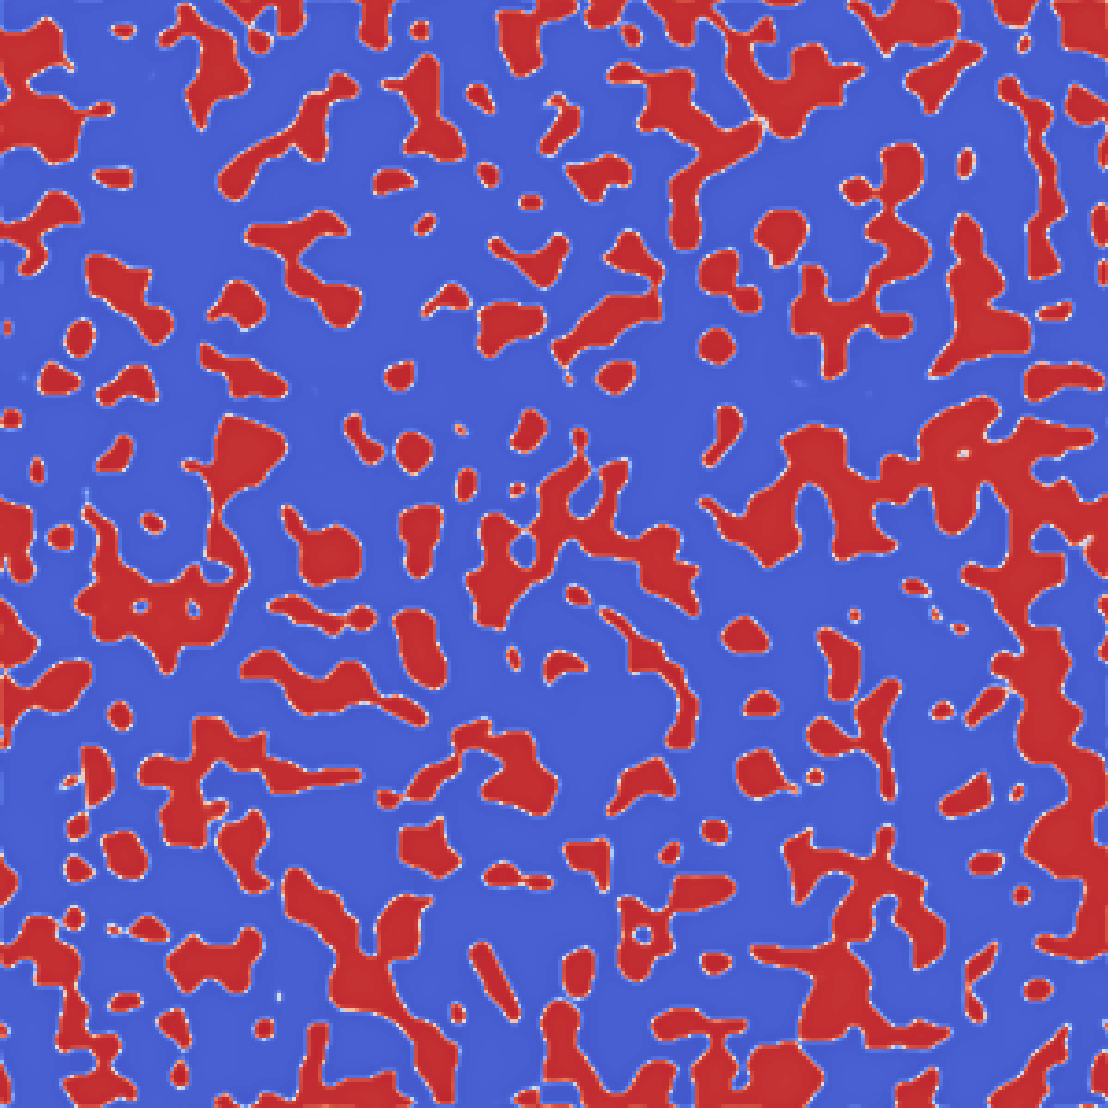
\includegraphics[width=0.32\linewidth]{papers/reaktdiff/images/FitzHughNagumo/fhn_n999.png}
    \caption{Verlauf der Simulation (Links nach Rechts) der Reaktions-Diffusiongleichung mit FitzHugh-Nagumo Modell(Gleichung \ref{reaktdiff:equ:fhn}) als Reaktionsterm}
    \label{reaktdiff:fig:fhn}
\end{figure}

Ein weiteres Model ist das FitzHugh-Nagumo Model.
Es wird genutzt um unteranderem die verbreitung von Nervenimpulse zu simulieren.
Die Reaktionsterme
\begin{equation}
    f(u,v) = \lambda_u u - u^3 - \kappa - \sigma v, \quad g(u,v) = \frac{1}{\tau}(u - v)
    \label{reaktdiff:equ:gs}
\end{equation}
Bilden Muster welche man in der Natur bei Tieren sehen kann.
Ein Beispiel ist in Abbildung \ref{reaktdiff:fig:gs} zu sehen.
\begin{figure}
    \centering
    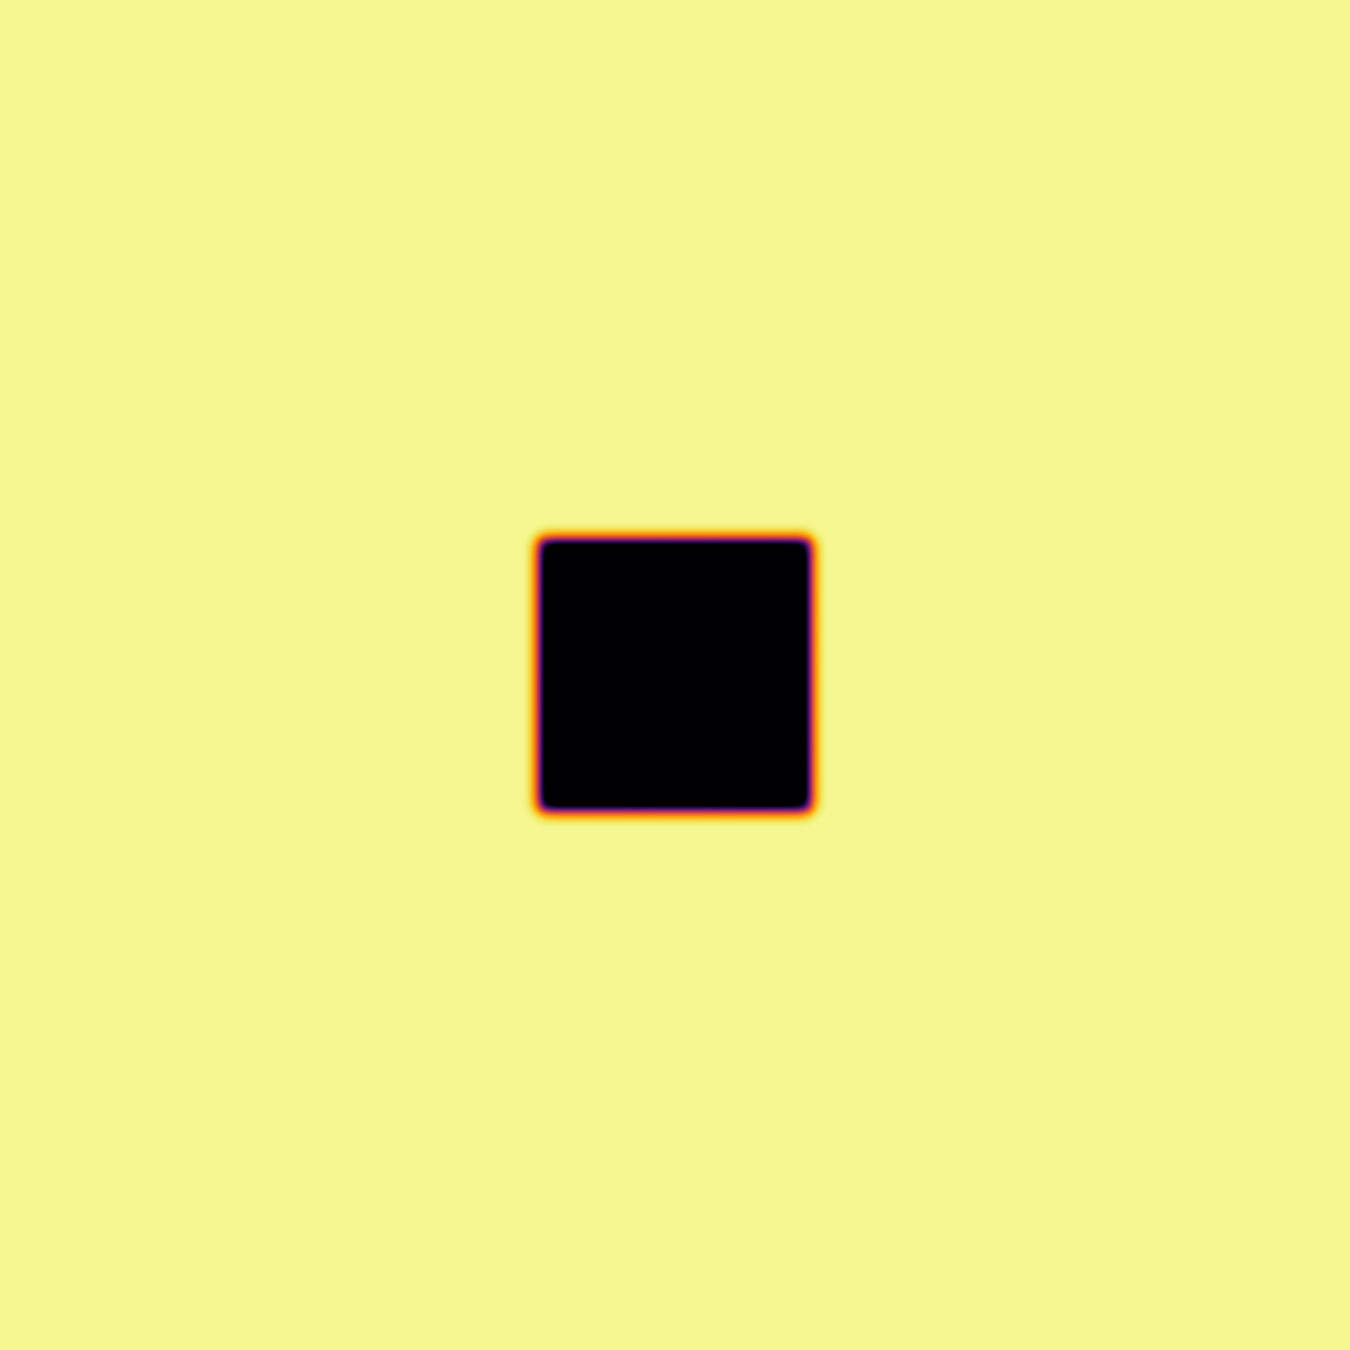
\includegraphics[width=0.32\linewidth]{papers/reaktdiff/images/GrayScott/gs_n1.png}
    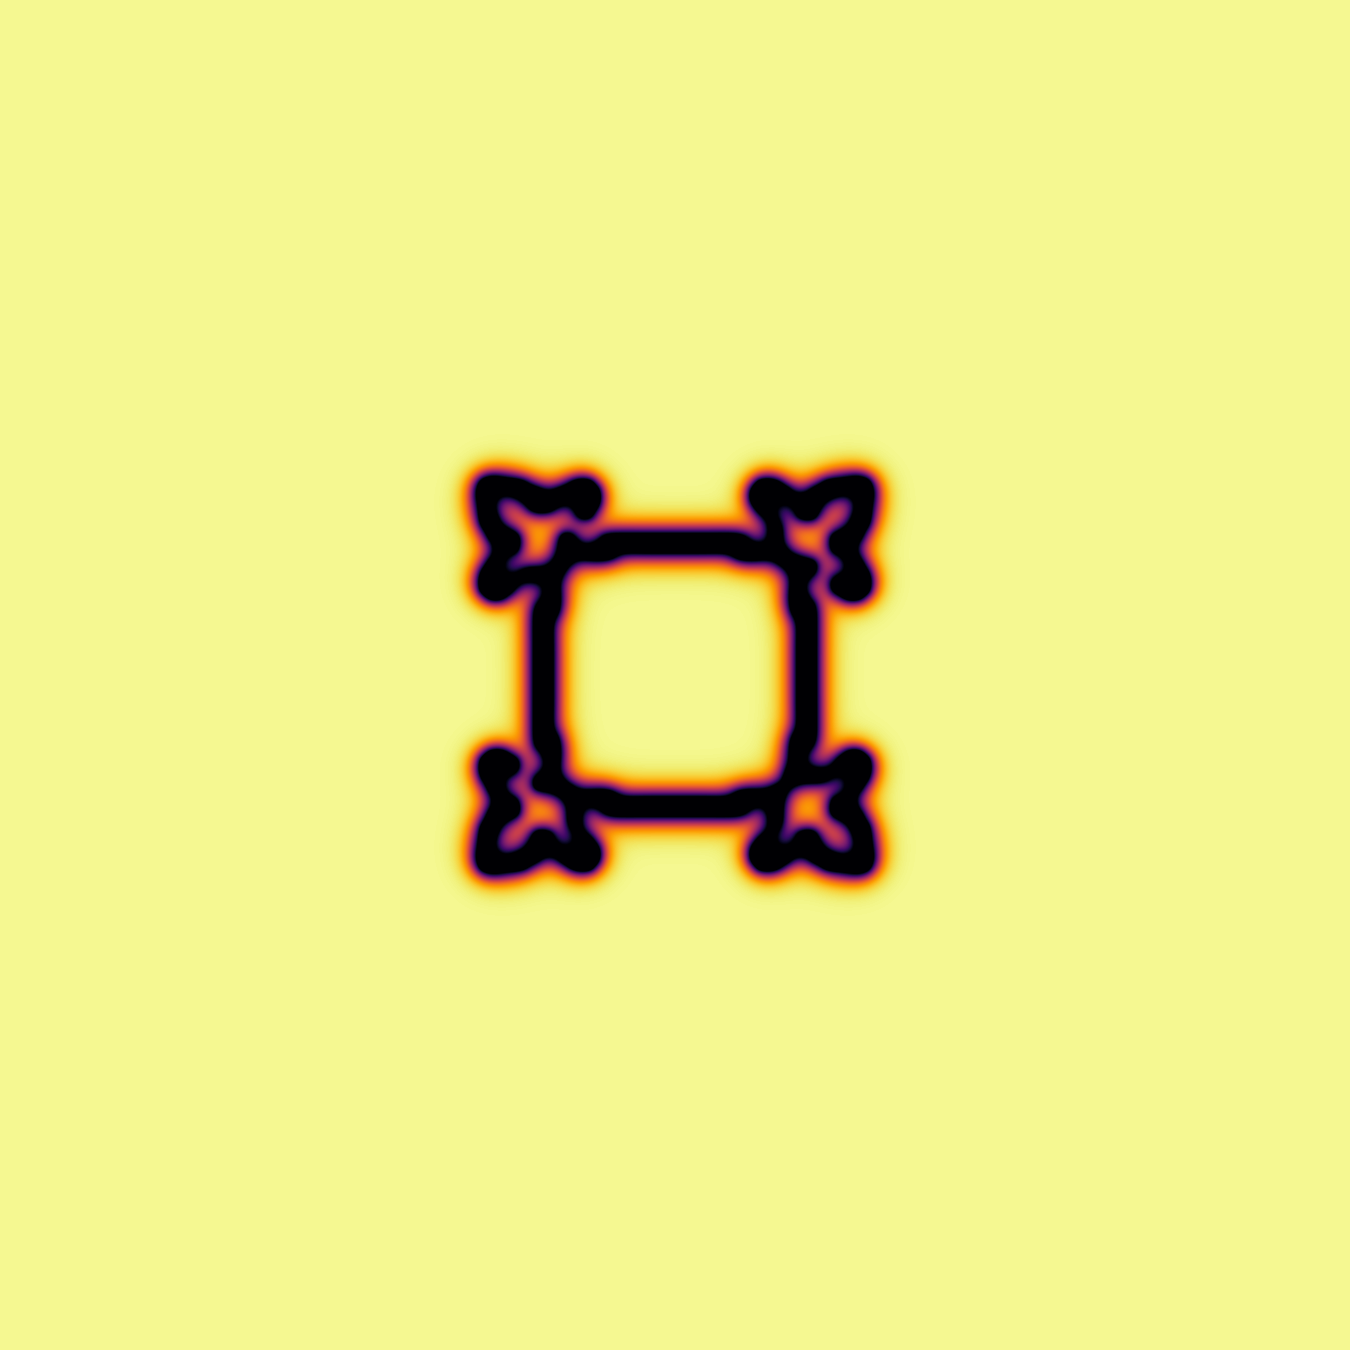
\includegraphics[width=0.32\linewidth]{papers/reaktdiff/images/GrayScott/gs_n300.png}
    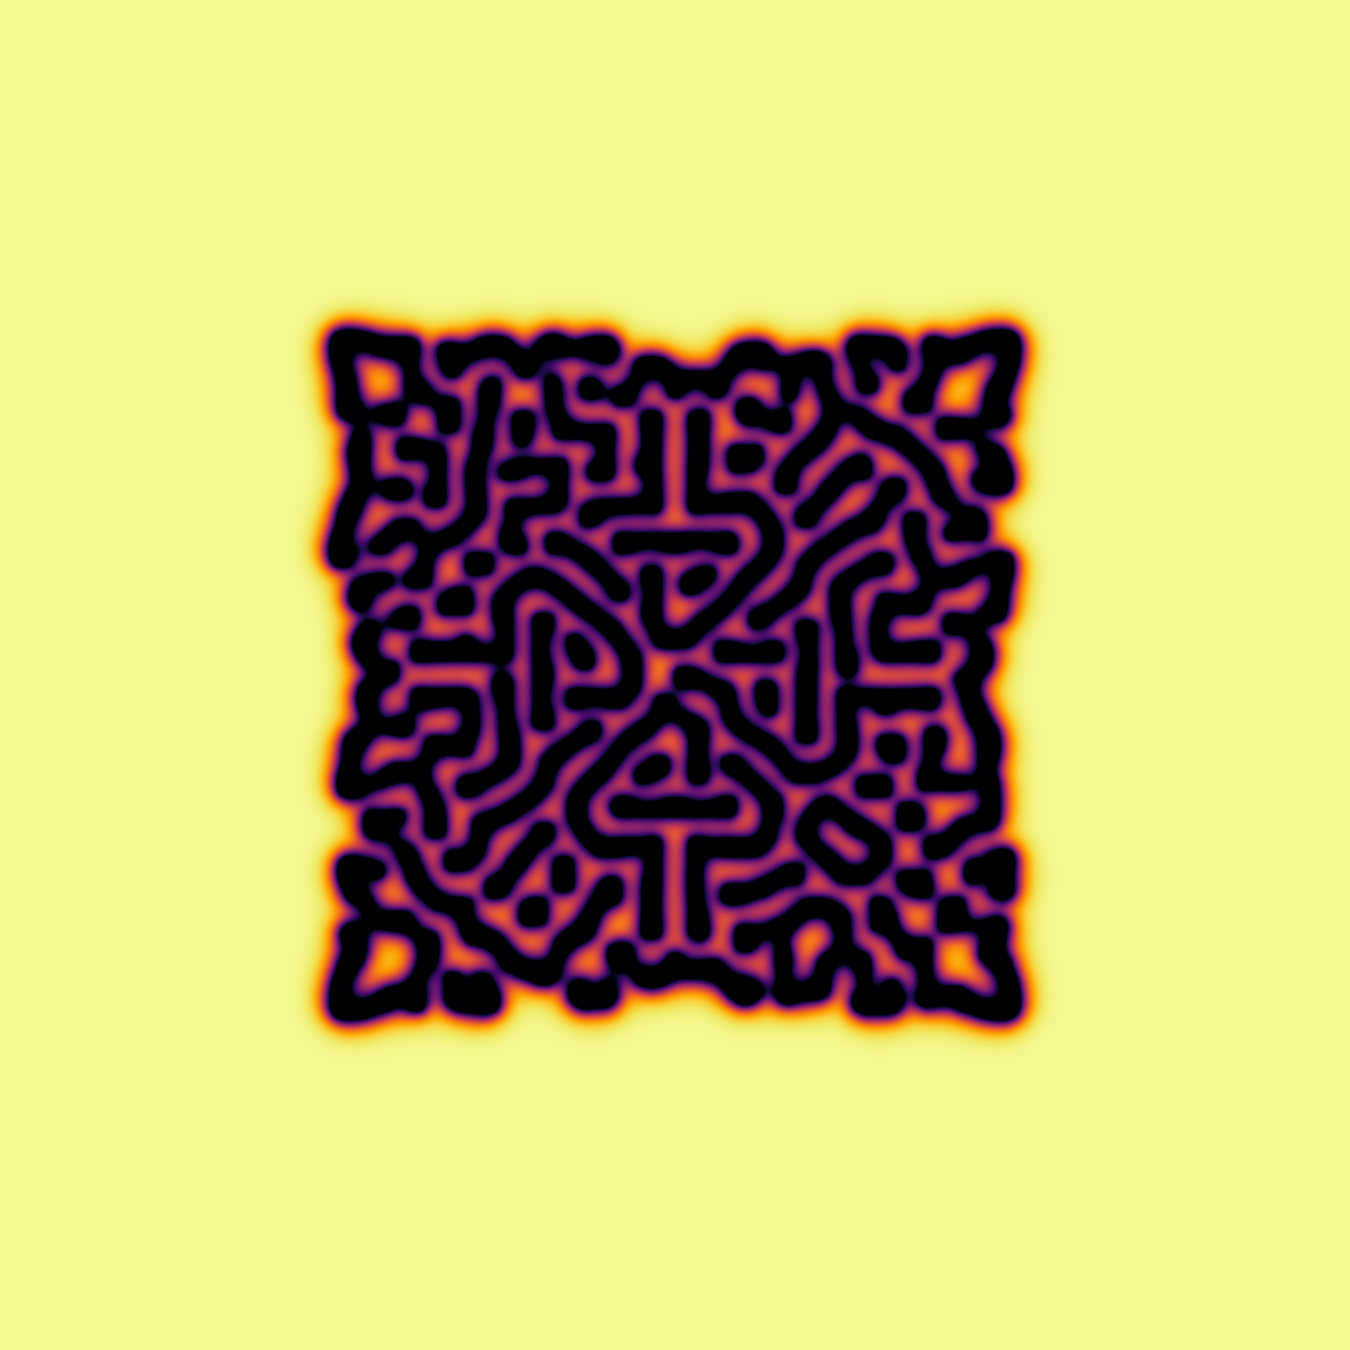
\includegraphics[width=0.32\linewidth]{papers/reaktdiff/images/GrayScott/gs_n999.png}
    \caption{Verlauf der Simulation (Links nach Rechts) der Reaktions-Diffusiongleichung mit Gray-Scott Modell(\ref{reaktdiff:equ:gs}) als Reaktionsterm}
    \label{reaktdiff:fig:gs}
\end{figure}
